\section{Introduction to Literature Review}
	\subsection{Readings for Literature Survey}
		This section will highlight some sources I have found that will most likely be of aid to my project; To start off; I 
		will need some form of text that can explain in detail the process of facial verification as well as image processing 
		concepts in general. To this end, I have highlighted ~\cite{szeliski2010computer} as one potential, probably invaluable, 
		source.  Another useful resource would be ~\cite{bradskeiLOCVwtOL} to provide a general overview to the usage of OpenCV. \\
		
		In order to run facial verification on a collection of images it would be wise to know how best to align the faces on 
		those images.  This is a process that falls under the aspect of normalization.  To help me figure out how this works I 
		have highlighted ~\cite{hasan2011improving} as possible useful information. \\
		
		Another aspect of normalization would be illumination normalization as stated I will be looking in-depth into the MIE 
		algorithm as proposed in~\cite{LuoaRINMBoMEfFR}.  \\
		
		Another area I would need to become proficient in would be mathematical optimization.  Namely, global optimization 
		techniques.  To help me with this I have highlighted ~\cite{Hungarian_alg}	as a possible method. \\
		
	\section{Overview of Used Systems}
		The toolbox is developed using Python and the OpenCV library in conjunction with the mathematical, 
		Numpy library.  However, too limit the scope of the project from getting too ambitious the system this 
		work implements will, at least initially, be console based. \\
		
		% OpenCV
		OpenCV is one of the most popular image processing libraries.  It was released under a BSD license 
		and thus is free for both academic and commercial use.  The provided functionality is highly optimised, 
		having been designed primarily for real-time computer vision.  The code base used to implement the 
		library functions is C/C++ to provide the most optimised solutions~\cite{OpenCVorg}.  \\
		
		% Python
		Python is an open source programming language designed for ease of use and learning.  It is an open 
		source project, hence free for use in any project you could need it for.  It is designed to interface 
		well with various aspects in computer science e.g. databases, web-servers, even other coding languages 
		with a relatively easy to use wrapping system to add in functionality provided in non-python libraries 
		for example the  afore mentioned OpenCV image processing library~\cite{Pythonorg}. \\
		
		\newpage
		% Numpy
		Numpy is a mathematical library focusing around matrix manipulations employing a powerful N-dimensional 
		array object.  It provides functionality to integrate C/C++ or Fortran code.  As with OpenCV it is licensed 
		under the BSD license and hence free for public or commercial use.  It is one of the prerequisites of OpenCV 
		in Python primarily because of its powerful matrix data representation, hence a good solution for a machine 
		representation of an image.  It permits its matrices to contain arbitrary data-types allowing ease and speed 
		of use in most database systems~\cite{Numpyorg}.
	
	\section{Image representation overview}
		The OpenCV library was chosen as it provides many useful image manipulation and computer vision techniques.  
		However, this means a solid understanding of how OpenCV represents these images is required to best make use 
		of the provided functionality.  \\
		
		OpenCV has already overloaded many mathematical operations to take their representation into account.  Hence 
		it is possible to simply take two images imported via ``cv.imread(...)'' or other such methods and add or 
		subtract them with a (``+'' or ``-'').  However, this is implemented only for basic mathematical operations.  When
		one wishes to perform more complex arithmetic procedures one needs to take into account the representation of 
		an image. \\
	
		The matrix representation that describes the images this work makes use of is that of a 
		simple 2D array or, mathematically, a 2D matrix.  This comprises the core of an image class.  However, there 
		are many other headers that are provided by an image class, these include headers that describe the width and 
		height of the image, the mathematical representation of the values inside the matrix (i.e. 8,16,32 bit numbers 
		weather or not they are floats etc), name of the image, how many channels it has i.e. (Red, Blue, Green) and whether 
		or not it has an alpha channel (transparency).  These comprise the most important features of an image
		~\cite{bradskeiLOCVwtOL}.\\
		
		\newpage
		It is noted that OpenCV makes use of Numpy, a mathematical matrix library, for many of its built-in procedures.  
		This is possible as OpenCV interprets the way Numpy represents matrices as images.  Thus is useful to client
		programs as Numpy can thus be used to take care of the heavy lifting with regards to manipulating an image's pixel 
		data.  This provides the client with a simple view of an image as a 2d array that can be manipulated as such.
		
		
		\section{Eigenface Algorithm}
			\subsection{Intuitive description}
			One of the most popular object recognition algorithms makes use of the mathematical eigenvector/principle 
			analysis for component analysis PCA is already implemented in OpenCV specifically for faces and is called 
			the Eigenface method. \\
			
			The Eigenface method of facial recognition works by taking the high dimensional face images represented 
			mathematically as an $m \times n$ matrix.  Providing it with N such images it takes them and finds the 
			average of the matrices(images) i.e. sum them together pixel by pixel and divide by N.  With this ``Average 
			face'' new images are created by subtracting the training images from the average image.  This represents each 
			face as a difference, or deviation from the average.  Once this has been done a set of orthonormal basis 
			matrices are calculated.  Each difference face can then be projected onto the bases, resulting in a feature
			vector of co-efficients which best represent these ``difference faces''.  Indeed, once a system is trained with 
			a set of images, given any of these training images one should be able to get coefficients that reconstruct 
			the original face exactly.  The reconstruction is done by adding the average face plus a linear combination 
			of the basis matrices.  The feature vector obtained determines the weighting of each basis matrix to enable 
			complete reconstruction of the training face. \\ 

			With these we can construct a face that somewhat represents one of the individuals we used in our training 
			set by taking the average face and adding varying components, determined by	a set of coefficients, of our 
			basis images.  This set of coefficients is called the feature vector of the difference face providing us the 
			means of recognition, as for similar faces (presumably of the same person) the feature vectors will be very 
			close.  
		
			\subsection{Training}
			The Eigenface method requires training, this means that it needs to be given images 
			of the faces it should recognize.  For example the set of faces shown in figure ~\ref{fig:Face_set}:
			
			\begin{figure}[h!]
				\centering
				\caption{Example of a training set.  Some faces are blacked out due to lack of permission.\label{fig:Face_set}}
				\includegraphics[width=105mm,height=105mm]{training_set_permitted.png}
			\end{figure}
			
			It then takes each image and converts it into a high dimensional vector created as: 
			
			\[ 		\Gamma_n = (Width)\times(Height) \quad | \quad n = 1,..,N \]
			
			Where N is the number of training images you have.	the result is a set {S} of N such face 
			image matrices: 			
			
			\[		S = {\Gamma_1,\Gamma_2,\Gamma_3,...,\Gamma_N} 		\]	
			
			After this is done the method finds the average face given as:											
			
			\[		\varphi = \frac{1}{N} \sum_{n=1}^{N} \Gamma_n  			\] 
			
			The average face constructed from this training set can be seen shown below in Figure ~\ref{fig:Ave_face}:
			
			\begin{figure}[h!]
				\centering
				\caption{The Average Face\label{fig:Ave_face}}
				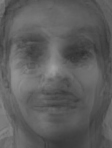
\includegraphics[width=200px,height=270px]{mean_image.png}
			\end{figure}
			
			Once the ``average face'' is determined the method calculates the difference $\phi$ between it and 
			each image in the training set.

			\[ 		\phi_n	=  \Gamma_n - \varphi						\]  
			
		
			We next obtain the covariance matrix C which we need for its Eigenvectors/values ($v_{n}, \lambda_{n}$) 
			respectfully. We obtain C via:
			
			\[		C 	= \frac{1}{N} \sum_{n=1}^{N} \phi_n \phi_n^T 	\] 	
			\[			= AA^T											\]

			where:
			\[ 		A = {\phi_1 , \phi_2, \phi_3, ... , \phi_n} 		\]

			\emph{Note, the superscript T implies the corresponding matrix/vector is transposed.}			
			
			The core concept of Eigenvector/value pairs is that given a matrix operation (in our case C) 
			on a vector ($v_{n}$) then this is equivalent to some scalar ($\lambda_{n}$) multiplied by that same vector. 
			
			\[		C v_{n} = \lambda_{n} v_{n} \quad n = 1,2...,N 		\]
			
			This relation allows us to find $v_{n}$ and $\lambda_{n}$ of C.  We create a new matrix $\omega$ by 
			combining these eigenvectors ($v_{n}$) ordered in descending eigenvalues ($\lambda_{n}$).  
			We then use this new construct to determine our feature vectors for each training face. via:			
			
			\[		y_n = \omega^T(\phi_n) 	\quad 	n = 1,2...,N 		\]
			
			Where $\phi_{n}$ as seen above is the difference image between the training image $n$ and the average image $\varphi$
			Note: although $\phi$ represents an image, mathematically we are viewing it as a single line vector.  We multiply this 
			vector by our created matrix $\omega$ to yield the feature vectors $y_n$ for our training data.  Thereafter we compare 
			any future image against these vectors to determine who they best match against.
			
		
			\subsection{Prediction}
			Once the recognizer has been trained with the input training data, what it stores are the average face, orthonormal basis 
			matrices and the feature vectors for each individual in the training data.  Then it can be fed some unseen images of the
			people it has trained on and see how it fares.  Herein we describe the procedure of taking a new image and testing it against 
			our trained recognizer. \\  
			
			To transform a new face into its Eigenface components.  First, subtract our input image $\Gamma$ from our mean image 
			$\varphi$ then multiply by the eigenvector matrix $\omega$.  Doing so, we produce the feature vector $x$:		
			
			\[		x = \omega^T(\Gamma - \varphi) \]
			
			We now determine which of the training faces is the best fit by finding the feature vector of the training face $y_n$ with the 
			minimum euclidean distance to the feature vector of the probe face $x$ we do so by calculating all these differences $\varepsilon_n$:
			
			\[			\varepsilon_n = \| x - y_n \|	\] 
			
			Then take:
			\[			min(\varepsilon_n)	\]
			
			To get the best match to our training data.  This distance also offers a means of indicating the confidence of this match. \\
			
			It should be added that Euclidean distance is not the only means of determining how different vectors are.  Indeed, for our 
			purposes it is possible that it could even be detrimental to the recognition rates.  Another solution would be to use the 
			absolute distance.  This is still not 100\% ideal but it may not have as much of an effect on our accuracy scores. \\
			
			If $\varepsilon_n$ is below a certain threshold defined within the algorithm the face is 
			considered to be known and represented by $\Omega_n$.  If instead the  $\varepsilon_n$ is 
			above the threshold the image is determined not to be face from the training data or indeed 
			a face at all.  If the threshold value is chosen too small only very close approximations 
			to our training set will be accepted by the algorithm leading to a higher accuracy, at the 
			other end, if the threshold is too large the algorithm will generate many false positives.  
			If the image is a face you know belongs to one of your subjects but the system determines it 
			is an unknown, then you could subsequently identify the individual by other means and then choose 
			to add it into the set of known faces and repeat the training steps i.e. incorporate the latest 
			image of the individual into the system (Doing so may be appropriate under certain circumstances 
			eg. the subject gets a hair cut, shaves his beard etc).
			
			\subsection{Summary of EigenFaces}
			So in summary, the Eigenface algorithm is provided with a set of face images to train on, then 
			once it is trained it is given an image, presumably a face of one of the people from the training 
			set, it will then ideally match it to the correct person and report how close the two feature 
			vectors are to each other are in the space provided.  \\
			
			It is important to note even though this method is called the Eigenface method, nothing about 
			it forces the use of facial images, indeed it is simply a image recognizer that has been shown 
			to work well on faces.  An example of PCA systems being used on non-face objects can be seen in
			~\cite{plantClassification} where they use the idea to identify different plant types based on 
			individual leaves from each plant.  One known weakness is that lighting will have a very large 
			impact on its performance, as opposed to other methods.  Though in other methods lighting does 
			play a part and is something you wish to remove, it is highly detrimental to the Eigenface method. 
			Thus to build a robust system lighting will need to be normalized and compensated for. \\
		
			The above mathematical understanding of the implementation of the Eigenface algorithm was 
			achieved via the tutorial found at~\cite{urlEgienFaceTut}.  Matthew Turk and Alex Pentland 
			developed the original algorithm~\cite{turk1991eigenfaces}.

	\section{Normalization}
		\subsection{Cropping}
		As has been stated the Eigenface algorithm is an image recognizer, thus background image 
		data will have a drastic impact on its performance and recognition rates.  For this reason 
		it is important to get rid of as much of an images background as possible.  
		Cropping an image is easy by hand, but the point of this whole exercise is to automate 
		the process of facial recognition as much as possible.  Hence, to crop a face out 
		of an image the face would first need to be found.  To this end, we would need a face 
		identifier. \\
		
		This work already implements such a feature in a separate component of the project ~\cite{MarceloFIFLA}.  
		As this work attempts to create a facial recognition tool-kit, the client can specify the bounds 
		of the cropping procedure once the face is found giving said user the ability to crop it 
		aggressively or not at all. \\
		
		Preliminary testing does indeed show that cropping an image has an effect on the recognition 
		rate.  However, these have been manual crops that do not resize the image nicely.  Also, some 
		faces are simply not well cropped with a lot of background left in the image.  Another improvement 
		that can be attempted is to white/black out the remaining background so that for all images the 
		background makes the same contribution to the algorithm's scoring system. 
		
		\subsection{Lighting}
		Lighting plays a very integral role for the Eigenface algorithm.  As such, we expand upon this concept
		more fully in chapter 3 by providing a strong background as to why lighting is an issue and experimenting 
		with various ways to overcome said issues posed by illumination. 
		
		\subsection{Alignment and scaling}
		The final big normalization issue would be face alignment and scaling, when a photo is taken/camera is 
		run, the faces wont be all similarly scaled or aligned.  This is something the system needs to take
		into account. \\
		
		Hence this becomes a software problem.  Most alignment algorithms find suitable features in a face with 
		which to re-align the face correctly~\cite{hasan2011improving}.  Such features can include the location 
		of the eyes in a face and use these to re-align the head so that it is as straight on as possible.  This 
		could be achieved by taking the eyes, drawing a line between them and levelling this line out so that it 
		is straight.  It should be noted that the nose can also be used as an alignment feature but the eyes are 
		favoured as they provide a longer axis to align with.  \\
		
		Scaling of a face can also be achieved through the distance between the eyes.  The image as a whole 
		can be scaled bigger or smaller so that this distance conforms to a fixed value. 	
		
\section{Summary}
	This work aims to create a facial detection and recognition tool-kit.  However, the true extent of this goal 
	is beyond the scope of this paper.  The main goal of this work, at least initially, is to get an end-to-end 
	system up and running even if many features require manual input.  For example; cropping and alignment can be 
	done by hand by prompting the client to locate the centre of the eyes in an image.  Taking these locations, it
	can realign the head and set the eyes to fixed locations. \\
	
	The bulk of the current work focusses on the Eigenface algorithm for facial recognition.  More importantly, 
	it attempts to fully understand and implement the normalization technique called the Mean Illumination 
	Estimation~\cite{LuoaRINMBoMEfFR} and ascertain the benefit on Eigenfaces accuracy rating by using this 
	pre-processing technique. \\
	
	As was explained earlier a key aspect of the system is that its framework and structure will be easy to extend 
	and utilise.  Providing future researchers with the ability to add the functionality they desire whether they 
	wish to add extra pre-processing methodologies or a more robust recognition algorithm.